\documentclass[11pt]{article}
\usepackage{latexsym}
\usepackage{amsmath}
\usepackage{amssymb}
\usepackage{amsthm}
\usepackage{epsfig}
\usepackage{graphicx}

\newcommand{\handout}[5]{
  \noindent
  \begin{center}
  \framebox{
    \vbox{
      \hbox to 5.78in { {\bf CSCE 643 } \hfill #2 }
      \vspace{4mm}
      \hbox to 5.78in { {\Large \hfill #5  \hfill} }
      \vspace{2mm}
      \hbox to 5.78in { {\em #3 \hfill #4} }
    }
  }
  \end{center}
  \vspace*{4mm}
}

\newcommand{\topic}[4]{\handout{#1}{#2}{#3}{Scribe: #4}{Topic #1}}

\newtheorem{theorem}{Theorem}
\newtheorem{corollary}[theorem]{Corollary}
\newtheorem{lemma}[theorem]{Lemma}
\newtheorem{observation}[theorem]{Observation}
\newtheorem{proposition}[theorem]{Proposition}
\newtheorem{definition}[theorem]{Definition}
\newtheorem{claim}[theorem]{Claim}
\newtheorem{fact}[theorem]{Fact}
\newtheorem{assumption}[theorem]{Assumption}

% 1-inch margins, from fullpage.sty by H.Partl, Version 2, Dec. 15, 1988.
\topmargin 0pt
\advance \topmargin by -\headheight
\advance \topmargin by -\headsep
\textheight 8.9in
\oddsidemargin 0pt
\evensidemargin \oddsidemargin
\marginparwidth 0.5in
\textwidth 6.5in

\parindent 0in
\parskip 1.5ex
%\renewcommand{\baselinestretch}{1.25}

\begin{document}

\topic{1 -- The Configuration Space}{Feburary 6th, 2025}{Prof. \ Dylan Shell / Dr. Steven Lavelle}{David Zhang}



\section{Overview}

\begin{definition}
  \textbf{Configuration Space: }The state space for motion planning is a set of possible transformations that could be applied to the robot
\end{definition}

\section{Basic Topological Concepts}

\subsection{Topological Spaces}

\begin{definition}
  \textbf{An open set is } a interval with no boundary points. That must follow this rule (TLDR) 
\end{definition}

\begin{definition}
  \textbf{A topological space} is a set $\mathbb{X}$ together with a collection of open sets $O$ that satisfy the following properties:
  \begin{enumerate}
    \item The union of any number of open sets is an open set.
    \item The intersection of a finite number of open sets is an open set
    \item Both $\mathbb{X}$ and $\emptyset$ are open sets
  \end{enumerate}
\end{definition}

\begin{definition}
 \textbf{Special Points: } A point on the border of an open or closed set
\end{definition}

\subsubsection{Special Point scenarios}
Consider a point $x$ that in the topological space $\mathbb{X}$, and a set $U$ that is a subset of $X$. The following terms
capture the position of point $x$ relative to U.
\begin{enumerate}
  \item If $x$ is in $U$, then $x$ is an interior point of $U$
  \item If $x$ is not in $U$, then $x$ is an exterior point of $U$
  \item If $x$ is neither an interior point nor an exterior point of $U$, then $x$ is a boundary point of $U$
  \item If $x$ is an interior or boundary point, it is a limit point (which the set of all limit points of $U$ 
  is called the closure of $U$)
\end{enumerate}

\em Important Note: The closure is always a closed set, because it contains all the boundary points. That also means
the open set contains none of the boundary points, making it open.

\subsection{The Ball analogy (Example 4.1)}
Think of an open set as a ball in $\mathbb{R}^n$ space, and the points that fill the ball are the interior points
centered at some point $x$.

\begin{enumerate}
  \item All open sets can be represented by a countable union of open balls
  \item Any function constructed from primitives that use the $<$ relation are open.
\end{enumerate}

\subsection{Subspace Topology}
The subspace topology is a topology that have all of its representative open sets be every subset to a larger 
topological space. $U \subseteq \mathbb{X}$

\begin{definition}
  \textbf{Hausdorff axiom:} For any distinct points $x_1$ and $x_2 \subseteq X$, there exists open sets
  $O_1$ and $O_2$ such that $x_1 \in O_1$ and $x_2 \in O_2$ and $O_1 \cap O_2 = \emptyset$
\end{definition}

In other words, points can be separated into distinct non-overlapping subsets.

\begin{definition}
  \textbf{Homeomorphism:} A function $f: \mathbb{X} \rightarrow \mathbb{Y}$ is a homeomorphism if it is bijective, and
  the function and its inverse are both continuous. Two topological spaces $X$ and $Y$
  
  If two topological spaces $X$ and $Y$ are homeomorphic, then they are topologically equivalent, which means there exists a homeomorphism between them.
  This property is reflexive, symmetric, and transitive.

\end{definition}
\begin{definition}
  A topological space is bounded if there exists a ball $B \subset \mathbb{R}^n$ if there exists a ball
  $B \subset \mathbb{R}^n$ such that $X \subset B$. 

\end{definition}
\begin{fact}
  The mapping $x \rightarrow \frac{1}{x}$ makes two open sets $(0, 1)$ and $(1, \infty)$ homeomorphic.  
\end{fact}

\begin{definition}
  \textbf{Topological Graph:} A graph for which every vertex corresponds to a point in $X$ and every edge corresponds
  to a continuous, injective function from $\tau : [0, 1]$ to $X$.
\end{definition}

\begin{definition}
  Two graphs are \textbf{isomorphic} if there exists a bijective mapping, $f: V_1 \rightarrow V_2$ such that there 
  is an edge between $v_1$ and $v_2$ if and only if there is an edge between $f(v_1)$ and $f(v_2)$ in the second graph.
\end{definition}

% Insert isomorphic_graph.png here
\begin{figure}[h]
  \centering
  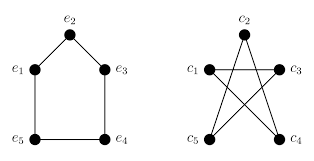
\includegraphics[width=0.35\textwidth]{isomorphic_graph.png}
  \caption{Isomorphic Graph Example}
\end{figure}



\subsection{Manifolds}

\begin{definition}
  \textbf{Manifold:} A topological space $M \subseteq \mathbb{R}^m$ is a manifold if for 
  every point $x \in M$, there exists an open set $O \subset M$ such that $O$ is homeomorphic to an open set in $\mathbb{R}^n$.
   $x \in O$ and $O$ is homeomorphic to an open set in $\mathbb{R}^n$. $n$ is the dimension of the manifold.

  In simple terms, it behaves at every point like our intuitive notions of a surface.
\end{definition}

\begin{corollary}
  This naturally leads to $m \geq n$ leading to whitney's embedding theorem. 
\end{corollary}

\section{What is a manifold?}

A topological space that is "understood" is a manifold. 
\begin{observation}
  $S^1$ is a circle.
  \begin{itemize}
    \item The circle can be stretched and deformed, into a square, so they are topologically equivalent
    \item As long as we don't cut or pinch the circle, they are equivalent (homeomorphic)
  \end{itemize}
  $S^2$ is a sphere.
  \begin{itemize}
    \item A sphere lives in 3-D Space
    \item $S^2$ is embedded in topological 3D space
  \end{itemize}

  Note: A torus is not topologically equivalent to a sphere, because it has a hole in it.
\end{observation}

\begin{definition}
  \textbf{Charts:} A chart is a cover of a topological space that gives coordinates to the space.
  They map a part of the manifold that to $\mathbb{R}^d$.
\end{definition}

Consider the earth as a manifold, the set of all locations on the earth. Of which we can problem sections of the earth
as maps. And collections of these maps are called atlases. The maps are 2D images of the manifold to represent a
3D space. The altas may have portions of the map that overlap. 

\begin{definition}
  $\mathbb{S}^1 = \{x \in \mathbb{R}^2 | x_1^2 + x_2^2 = 1\}$ \\ 
  It is a circle.
\end{definition}

\subsubsection{Identification in manifolds}
\begin{definition}
  \textbf{Identification:} A general method of declaring that some points of a space are identical even though they originally were 
  distinct.
\end{definition}

\begin{figure}[h]
  \centering
  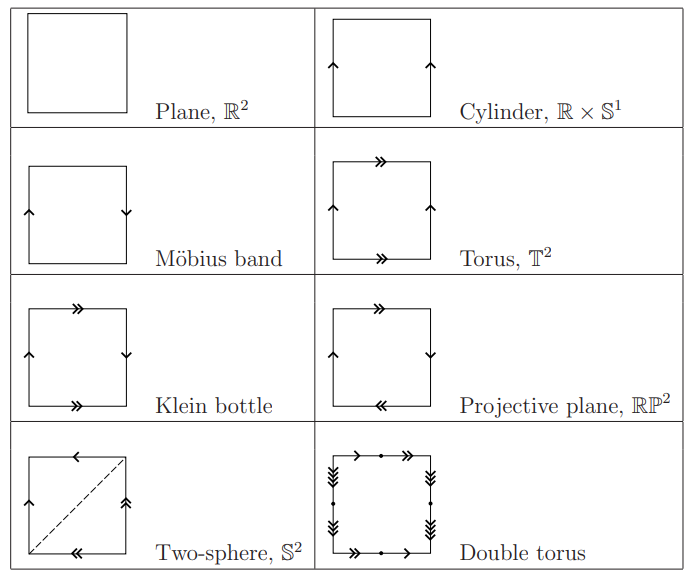
\includegraphics[width=0.5\textwidth]{2D_manifolds.png}
  \caption{Identification Example}
\end{figure}

The figures showcase sections of a manifold and their identification.
Arrows represent the mapping of the points. For example, for the cylinder, the top and the bottom are linked together
mapping $(0, y) ~ (1, y)$.

\subsection{Paths and Connectivity}
We essentially want to \textbf{connect one part of space to another part of space}, and we can do this by utilizing a 
sequence of actions. Graphs are for discrete spaces, and topological spaces are for continuous spaces.

\begin{definition}
  \textbf{Path:} A path is a continuous function from $\tau : [0, 1] \rightarrow X$.
  $\tau = x(s)$ where $x$ is the path and $s$ is the state index in the path.
\end{definition}

\begin{definition}
  \textbf{Connected Space:} A space is connected if there is a path or a union of two disjoint, nonempty, open sets.
\end{definition}
\begin{definition}
  \textbf{Homotopic Paths:} Two paths are homotopic if there exists a continuous function $h: [0, 1] \times [0, 1] \rightarrow X$
  such that the paths deformed into the other. There cannot be a discontinuous jump between the paths.
\end{definition}

This also leads into algebraic topology, which is mainly characterized by groups

\begin{definition}
  \textbf{A group} is defined by the 4 properties:
  \begin{enumerate}
    \item Closure - multiplication / binary operations are closed within the group
    \item Associativity - $(a \cdot b) \cdot c = a \cdot (b \cdot c)$
    \item Identity - There exists an identity element $e$ such that $a \cdot e = e \cdot a = a$
    \item Inverse - For every element $a$, there exists an inverse $a^{-1}$ such that $a \cdot a^{-1} = a^{-1} \cdot a = e$
  \end{enumerate}
\end{definition}

% TODO: Add more details from The Fundamental Group

\paragraph{Bibliography.}
Please give real bibliographical citations for the papers that we
mention in class. See below for how to include a bibliography section.
If you use BibTeX, integrate the .bbl file into your .tex
source. You should reference papers like this: ``The FKS
dictionary originates in a paper by Fredman, Koml\'{o}s and
Szemer\'{e}di \cite{fks}.'' In general, the name of the authors should
appear in text at most once (for the first citation); further
citations look like: ``Our proof follows that of \cite{fks}''.

Take a look at previous topics (TeX files are available) to see the
details. A excellent source for bibliographical citations is
DBLP. Just Google DBLP and an author's name.


%\bibliography{mybib}
\bibliographystyle{alpha}

\begin{thebibliography}{77}

\bibitem{fks}
M. Fredman, J. Koml\'{o}s, E. Szemer\'{e}di,
\emph{Storing a Sparse Table with $O(1)$ Worst Case Access Time},
Journal of the ACM, 31(3):538-544, 1984.

\end{thebibliography}

\end{document}